\newpage 

\section{Compiler Optimizations for Thread-Level Speculation}


While
using this multithreaded hardware to improve the throughput of a
workload is straightforward, using it to improve the performance
of a single application requires parallelization. The ideal solution
would be to convert sequential programs into parallel programs automatically, but unfortunately this is difficult (if not impossible) for
many general-purpose programs due to their use of pointers, complex data and control structures, and run-time inputs.


Thread-Level Speculation (TLS) [1, 6, 14, 15, 16, 20, 21, 26,
30, 34] is a potential solution to this problem since it allows the
compiler to create parallel threads without having to prove that
they are independent. The underlying hardware ensures that interthread 
dependences through memory are satisfied, and re-executes
any thread for which they are not.

The key to extracting parallelism from these programs and hence
improving performance is in the efficiency of speculative execution. 
While recent research has investigated hardware optimization
for TLS [6, 20, 22, 31, 24], there has been relatively little work
on compiler optimization in this area. One potential opportunity for optimization focuses on data dependences between speculative
threads that occur frequently: if the compiler is able to identify the
source and the destination of a frequent inter-thread data dependence, then it is beneficial to insert synchronization and forward
that value explicitly to avoid failed speculation. Figure 1(a) shows
an example loop that the compiler has speculatively parallelized by
partitioning the loop into speculative threads (aka epochs). Since
the variable A is read and written in every iteration, the compiler decides to synchronize and forward A by inserting a wait operation
before the first use of A, and a signal operation after the last definition of A—we describe, implement, and evaluate this algorithm
in Section 3. The synchronization results in the partially-parallel
execution shown in Figure 1(a), where each epoch stalls until the
value of A is produced by the previous epoch. The flow of the value
of A between epochs serializes the parallel execution, and so we refer to it as a critical forwarding path. In the next section, we show
that the overall performance of speculation is limited by the size of
this critical forwarding path.

\begin{figure}[H]
	\centering
	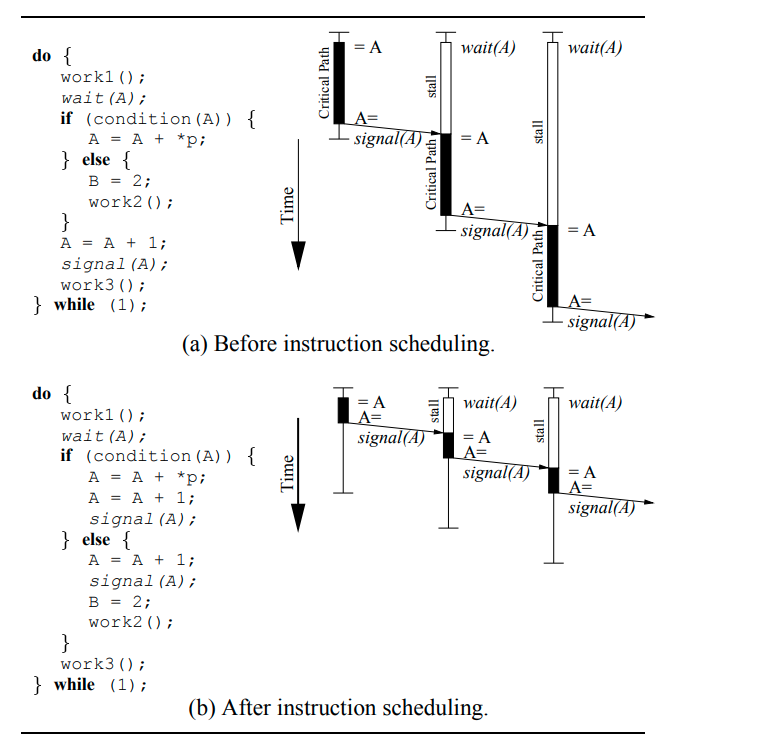
\includegraphics[width=0.3\textwidth]{p207.png}
	\caption{ Impact of scheduling on the critical forwarding path.}
	\label{fig:p207}
\end{figure}

\subsection{What Can the Compiler Do to Improve Performance?\cite{zhai2002compiler}}


Although synchronization is better than speculation for a data dependence that occurs frequently, the resulting serialization can still
limit performance. In fact, the performance of many applications
that exploit TLS is limited by the critical forwarding path. Figure 2
shows the potential impact of reducing the critical forwarding path
on a four-processor chip multiprocessor—we will explain the details of this experiment later in Section 2. The U bars show the
unscheduled TLS version of each application run speculatively in
parallel. Each bar is normalized to the execution time of the original sequential version, such that bars less than 100 are speeding
up. The best we can possibly do with scheduling is to eliminate
the critical forwarding path altogether. We measure this ideal behavior with a model that can perfectly predict all forwarded values
such that there is no synchronization (P). We see that for most applications, removing the synchronization bottleneck results in great
performance improvements.


\begin{figure}[H]
	\centering
	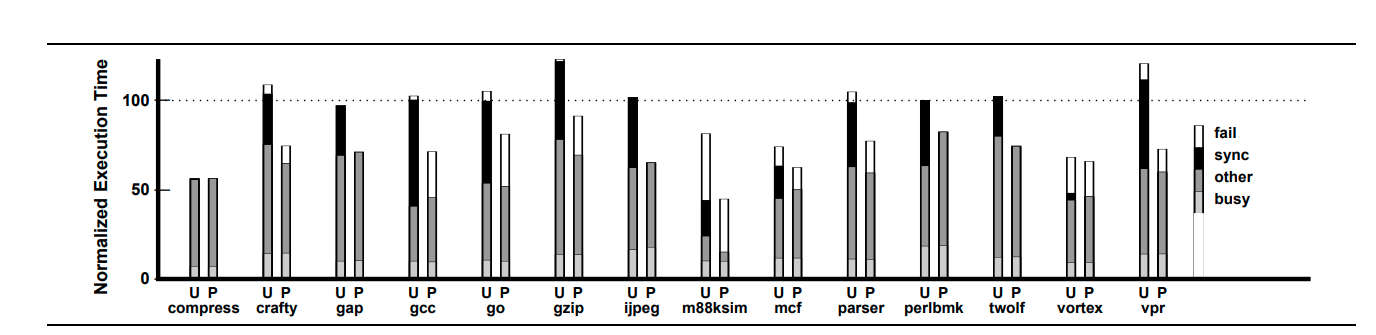
\includegraphics[width=0.8\textwidth]{p208.png}
	\caption{Potential impact of reducing the critical forwarding path. For each benchmark we show execution time on four processors for the speculatively parallelized regions of code normalized to that of the original sequential versions. U is the unscheduled
    speculative version and P shows the impact of perfect prediction of forwarded values.}
	\label{fig:p208}
\end{figure}


What can the compiler do to shrink the critical forwarding path?
The key idea is to reduce the number of instructions between each
wait/signal pair. However, this becomes more difficult in the
presence of conditional control flow. Figure 1(b) shows the example loop after the compiler has scheduled the code to reduce the
critical forwarding path. The scheduling algorithm has duplicated
the computation of A=A+1 as well as the signal and moved them
into the conditional structure. If the condition on A is rarely true,
then less work will be performed before reaching each signal (by
deferring the computation of B=2 and work2()). As shown in the
figure, this reduces the stall time for each epoch, thereby improving
overall execution time. 



\subsubsection{Inserting Wait/Signal}


\subsubsection{Scheduling Instructions}


\subsubsection{Scheduling Instructions Speculatively}







